\documentclass[12pt,a4paper]{article}
\usepackage[utf8]{inputenc}
\usepackage[spanish,es-tabla]{babel}
\usepackage{geometry}
\usepackage{graphicx}
\usepackage{multirow}
\usepackage{tabularx}
\usepackage{mathptmx}
\usepackage{fancyhdr}
\usepackage{array}
\usepackage[table]{xcolor}
\usepackage{titlesec}
\usepackage{setspace}
\usepackage{microtype}
\usepackage{lastpage}
\usepackage{booktabs}
\usepackage{enumitem}
\usepackage{amsmath}
\usepackage{amsfonts}
\usepackage{amssymb}

\graphicspath{{images/}{../images/}{./}}

\geometry{
    top=4.7cm,
    bottom=2.5cm,
    left=2.5cm,
    right=2.5cm,
    headheight=3.9cm,
    headsep=0.4cm
}

\setstretch{1.15}
\setlength{\parindent}{0pt}
\setlength{\parskip}{0.45em}
\setlength{\tabcolsep}{4pt}

\titleformat{\section}
  {\normalfont\fontsize{12}{14.5}\bfseries}{\thesection.}{0.6em}{\uppercase}
\titlespacing*{\section}
  {0pt}{1.8ex plus 0.4ex minus 0.2ex}{0.6ex plus 0.2ex}

\titleformat{\subsection}
  {\normalfont\fontsize{11.5}{13.5}\bfseries}{\thesubsection.}{0.5em}{}
\titlespacing*{\subsection}
  {0pt}{1.4ex plus 0.3ex minus 0.1ex}{0.4ex plus 0.1ex}

\titleformat{\subsubsection}
  {\normalfont\fontsize{10.5}{12.5}\bfseries\itshape}{\thesubsubsection.}{0.4em}{}
\titlespacing*{\subsubsection}
  {0pt}{1.1ex plus 0.2ex minus 0.1ex}{0.3ex plus 0.1ex}

\newcolumntype{Y}{>{\centering\arraybackslash}X}
\newcolumntype{L}{>{\raggedright\arraybackslash}X}
\newcolumntype{C}{>{\centering\arraybackslash}X}

\definecolor{headerred}{RGB}{180, 0, 0}
\definecolor{darkred}{RGB}{140, 0, 0}
\definecolor{lightgraybg}{RGB}{248, 248, 248}
\definecolor{tableheader}{RGB}{232, 238, 246}

\newcommand{\docCodigo}{TI-SIGE-ENT-S1-001}
\newcommand{\docVersion}{1.0}
\newcommand{\docProceso}{INGENIERÍA DE REQUERIMIENTOS / DIAGNÓSTICO AS-IS}
\newcommand{\docElaboracion}{14/08/2026}
\newcommand{\docRevision}{PENDIENTE DE REVISIÓN}
\newcommand{\docTitulo}{LEVANTAMIENTO DE INFORMACIÓN DEL PROCESO ACTUAL (AS-IS)}
\newcommand{\docOrganizacion}{FACULTAD DE INGENIERÍA EN SISTEMAS, ELECTRÓNICA E INDUSTRIAL}
\newcommand{\docSubOrganizacion}{CARRERA DE INGENIERÍA DE SOFTWARE}

\newcommand{\encabezadofrecuente}{%
    \renewcommand{\arraystretch}{1.15}%
    \noindent\makebox[\textwidth][c]{%
    \begin{tabularx}{\textwidth}{|>{\centering\arraybackslash}m{2.8cm}|Y|>{\centering\arraybackslash}m{4.8cm}|}
        \hline
        \multirow{4}{2.8cm}{\centering\raisebox{-1.15cm}{
\includegraphics[width=2.5cm,height=2.0cm,keepaspectratio]{images/logo.png}}}
        & \textbf{\fontsize{9}{11}\selectfont \docOrganizacion} 
        & \textbf{\fontsize{8}{10}\selectfont CÓDIGO:} \fontsize{8}{10}\selectfont \docCodigo \\
        \cline{3-3}
        & \textbf{\fontsize{8.5}{10.5}\selectfont \docSubOrganizacion} 
        & \textbf{\fontsize{8}{10}\selectfont VERSIÓN:} \fontsize{8}{10}\selectfont \docVersion \\
        \cline{2-3}
        & \textbf{\fontsize{8}{10}\selectfont PROCESO:} \fontsize{8}{10}\selectfont \docProceso 
        & \textbf{\fontsize{8}{10}\selectfont ELABORACIÓN:} \fontsize{8}{10}\selectfont \docElaboracion \\
        \cline{2-3}
        & \textbf{\fontsize{8.5}{10.5}\selectfont \docTitulo} 
        & \textbf{\fontsize{8}{10}\selectfont ÚLTIMA REVISIÓN:} \fontsize{8}{10}\selectfont \textbf{\textcolor{darkred}{\docRevision}} \\
        \hline
    \end{tabularx}%
    }%
}

\pagestyle{fancy}
\fancyhf{}
\fancyhead[C]{\encabezadofrecuente}
\fancyfoot[C]{\fontsize{10}{12}\selectfont Página \thepage\ de \pageref{LastPage}}
\renewcommand{\headrulewidth}{0pt}

\begin{document}

\section{Título}
\textbf{Denominación del Entregable:} Levantamiento de Información del Proceso Actual (Diagnóstico As-Is) -- Código EDT: 1.1



\section{Introducción}
En la Universidad Técnica de Ambato (UTA), y particularmente en la Facultad de Ingeniería en Sistemas, Electrónica e Industrial (FISEI), los procesos de planificación semestral y rendición de cuentas del cuerpo docente se rigen por el \textbf{Sistema de Gestión de Calidad (SGC)}. 

Actualmente, estos procesos se ejecutan mediante formatos estáticos en procesadores de texto (\texttt{.docx}) y hojas de cálculo (\texttt{.xlsx}) correspondientes a:
\begin{itemize}[leftmargin=1.5em, itemsep=1.5pt]
    \item \textbf{Formato Plan de Trabajo:} \texttt{UTA-SGC-A-2-1-P7-T1}
    \item \textbf{Formato Informe de Cumplimiento:} \texttt{UTA-SGC-A-2-1-P7-T2}
\end{itemize}

El presente documento formaliza el levantamiento de información y diagnóstico del estado actual (\textit{As-Is}), identificando las áreas de intervención, cuellos de botella y oportunidades de optimización para la solución web \textbf{SIGE}.

\section{Objetivo}

\subsection{Objetivo General}
Realizar el levantamiento de información y diagnóstico integral del flujo documental actual de elaboración, revisión y aprobación de planes de trabajo e informes institucionales del SGC en la FISEI UTA, identificando cuellos de botella y requerimientos base para el sistema SIGE.

\subsection{Objetivos Específicos}
\begin{itemize}[leftmargin=1.5em, itemsep=1.5pt]
    \item Mapear el flujo de actividades del proceso actual (\textit{As-Is}) desde la descarga de plantillas hasta la legalización en Consejo Directivo.
    \item Identificar y clasificar los principales problemas operativos, asimetrías de información y pérdidas de tiempo del personal docente.
    \item Relevar los formatos institucionales vigentes (\texttt{UTA-SGC-A-2-1-P7-T1} y \texttt{UTA-SGC-A-2-1-P7-T2}) y los catálogos de actividades académicas de la facultad.
\end{itemize}

\section{Alcance}

\subsection{Límites del Levantamiento (In-Scope)}
\begin{itemize}[leftmargin=1.5em, itemsep=1.5pt]
    \item Procesos de planificación e informes de docentes a tiempo completo y medio tiempo de las carreras de FISEI.
    \item Formatos oficiales de calidad SGC vigentes para el período académico 2026.
    \item Procedimientos de revisión de coordinadores de área y coordinadores de carrera.
\end{itemize}

\subsection{Exclusiones (Out-of-Scope)}
\begin{itemize}[leftmargin=1.5em, itemsep=1.5pt]
    \item Procesos de nómina y pagos financieros docentes.
    \item Trámites no académicos de índole administrativo-financiero central de la universidad.
\end{itemize}

\section{Definiciones}
\begin{itemize}[leftmargin=1.5em, itemsep=2pt]
    \item \textbf{SGC (Sistema de Gestión de la Calidad):} Conjunto de normas y formatos institucionales para asegurar la calidad académica en la UTA.
    \item \textbf{As-Is:} Diagnóstico de la situación operativa y tecnológica actual antes de la implantación de mejoras.
    \item \textbf{Plan de Trabajo (P7-T1):} Documento prospectivo donde el docente planifica sus horas y actividades del semestre.
    \item \textbf{Informe de Cumplimiento (P7-T2):} Documento retrospectivo donde se rinde cuentas de las horas ejecutadas con evidencias adjuntas.
    \item \textbf{FirmaEC:} Aplicativo oficial del gobierno ecuatoriano para firma digital con certificados PKCS\#12 o tokens criptográficos.
\end{itemize}

\section{Responsabilidades}
\begin{itemize}[leftmargin=1.5em, itemsep=2pt]
    \item \textbf{Analista de Requerimientos (Heidy Villavicencio):} Conducción de entrevistas, transcripción de hallazgos y consolidación de cuellos de botella.
    \item \textbf{Líder de Proyecto / Arquitecto (Steeven Toala):} Mapeo de procesos As-Is, diagramación de flujos y validación técnica del diagnóstico.
    \item \textbf{Docente Tutor (Ing. Paulo Torres):} Validación metodológica y aprobación del alcance del levantamiento.
\end{itemize}

\section{Normativa Legal y Técnica}
\begin{itemize}[leftmargin=1.5em, itemsep=2pt]
    \item \textbf{Reglamento de Régimen Académico CES:} Disposiciones sobre distribución del tiempo docente y dedicación horaria.
    \item \textbf{Norma ISO 9001:2015:} Requisitos para el control de la información documentada en organizaciones educativas.
    \item \textbf{Manual de Calidad SGC - Universidad Técnica de Ambato:} Directrices para el uso de plantillas P7-T1 y P7-T2.
\end{itemize}

\section{Método, Políticas y Contenidos}
Para el levantamiento se aplicaron tres técnicas de ingeniería de requerimientos:
\begin{enumerate}[leftmargin=1.5em, itemsep=2pt]
    \item \textbf{Entrevistas Semi-estructuradas:} Realizadas a 8 docentes titulares, 2 coordinadores de carrera y 1 delegado de la Comisión de Calidad.
    \item \textbf{Análisis de Artefactos y Documentación SGC:} Revisión exhaustiva de planes e informes históricos y de la matriz de propuestas de mejora de la facultad.
    \item \textbf{Observación Directa del Flujo Documental:} Seguimiento del trámite de un informe desde su elaboración hasta su legalización final en Consejo Directivo.
\end{enumerate}

\begin{figure}[htbp]
    \centering
    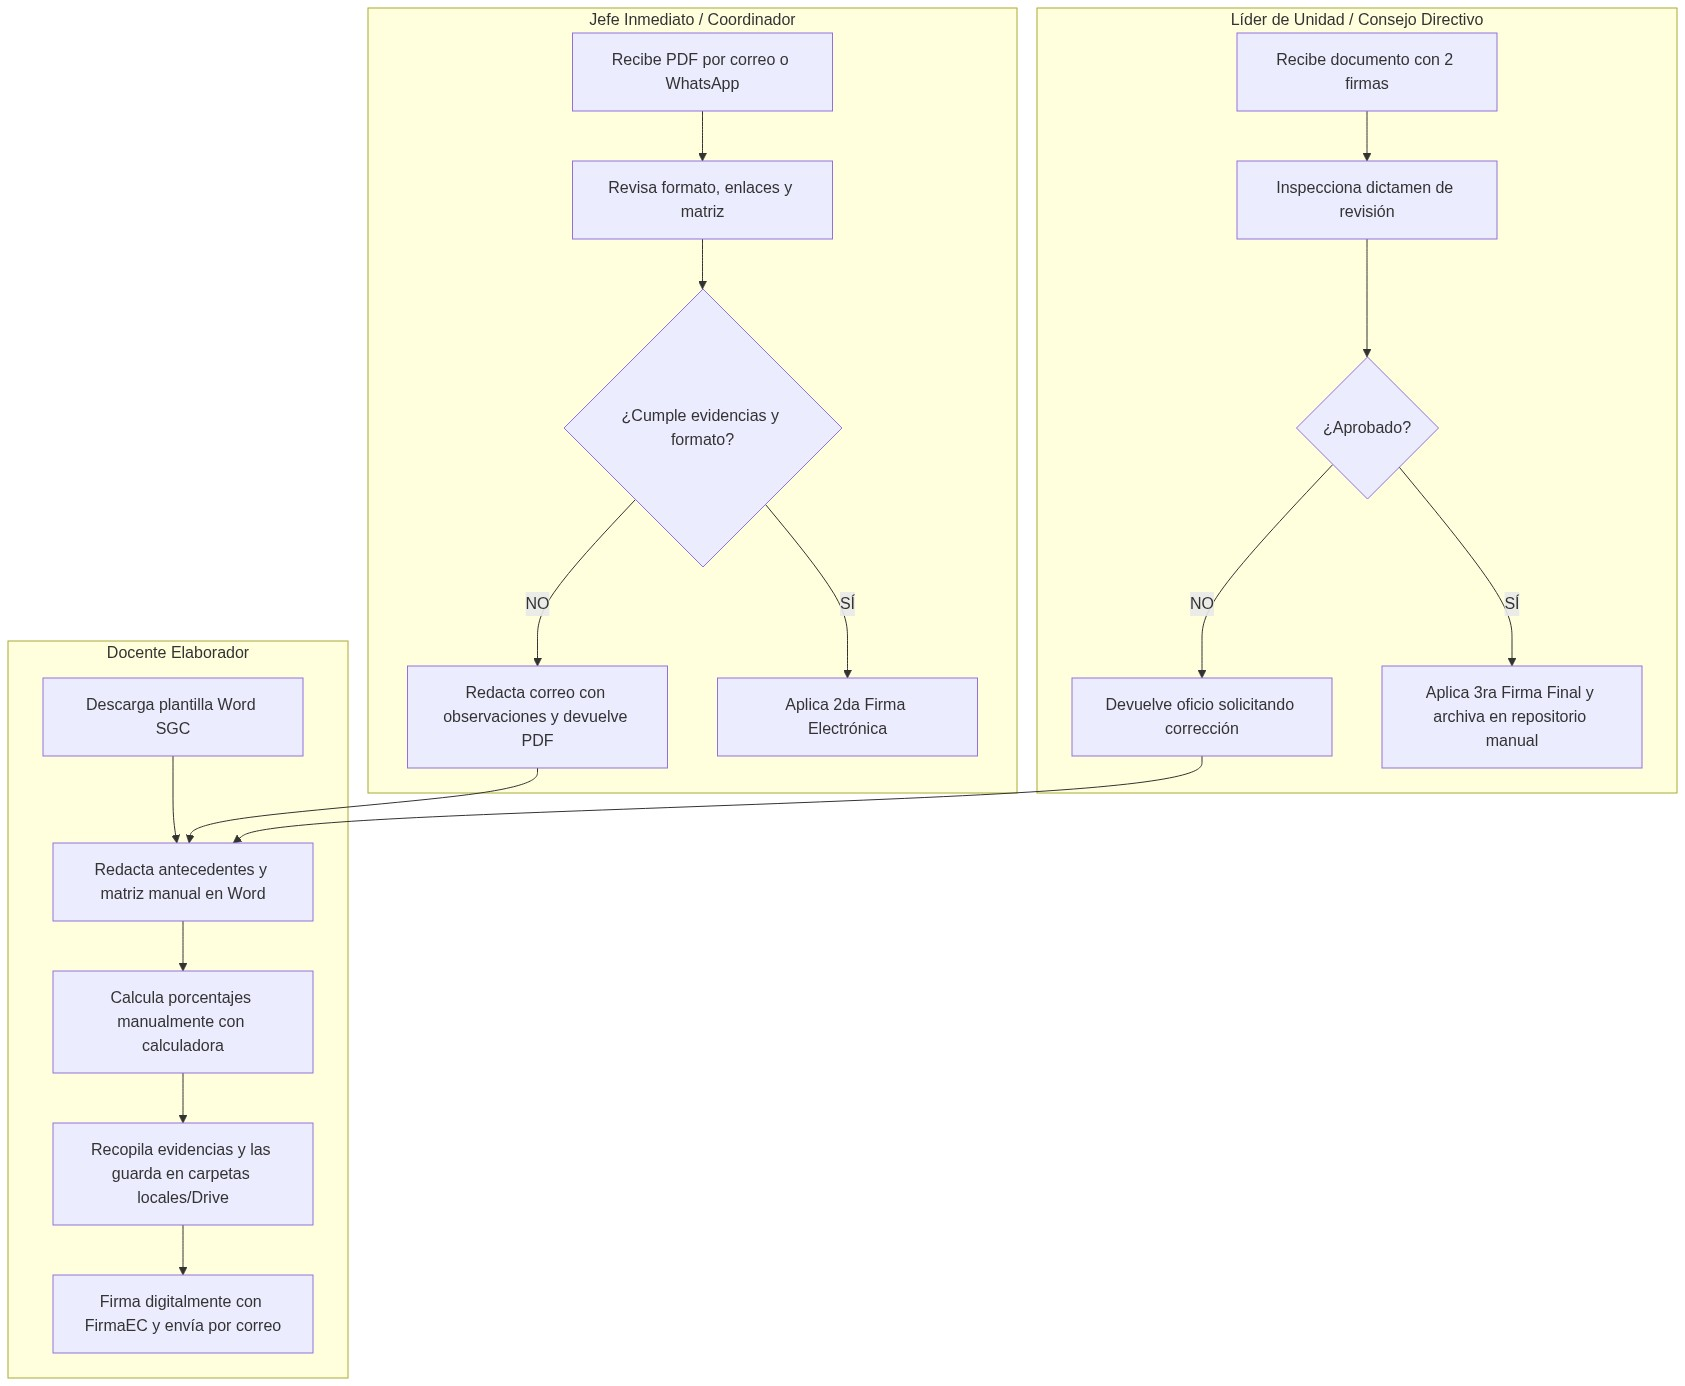
\includegraphics[width=0.85\textwidth,height=5.5cm,keepaspectratio]{images/s1_01_diagrama_as_is.png}
    \caption{Diagrama de Flujo del Proceso Actual As-Is (Elaboración y Aprobación Manual SGC).}
    \label{fig:s1_01_as_is}
\end{figure}

\section{Descripción de actividades}

\subsection{Diagnóstico de Problemas y Cuellos de Botella (P-01 al P-06)}

\begin{table}[htbp]
\centering
\small
\renewcommand{\arraystretch}{1.2}
\begin{tabularx}{\textwidth}{|c|>{\raggedright\arraybackslash\bfseries}m{3.5cm}|X|X|}
\hline
\rowcolor{tableheader}
\textbf{ID} & \textbf{Problema Identificado} & \textbf{Impacto Operativo} & \textbf{Evidencia Recopilada} \\
\hline
\textbf{P-01} & Asimetría de versiones y pérdida de trazabilidad & Confusión sobre cuál es el archivo final aprobado tras múltiples rondas de correcciones enviadas por email. & Se detectaron hasta 4 versiones distintas de un mismo informe circulando por correo. \\
\hline
\textbf{P-02} & Evidencias extraviadas o enlaces rotos & Informes aprobados sin medios de verificación adjuntos o con enlaces a Google Drive con permisos restringidos. & 35\% de los informes históricos analizados no poseían evidencias accesibles para auditoría. \\
\hline
\textbf{P-03} & Cálculo manual e inconsistencias en matrices & Errores aritméticos en sumas de ponderación que no totalizan el 100\% o avances incongruentes sin justificación. & Discrepancias entre las horas asignadas y los porcentajes reportados. \\
\hline
\textbf{P-04} & Sobrecarga de tiempo administrativo & El docente invierte un promedio de \textbf{8 horas hombre} por informe en tareas repetitivas de formateo y transcripción. & 1,800 horas anuales invertidas por el cuerpo docente en burocracia documental. \\
\hline
\textbf{P-05} & Fechas y períodos vulnerables a manipulación & Inconsistencias temporales entre la fecha de ejecución de la actividad y la fecha declarada en el informe. & Fechas redactadas a mano sin control de servidor. \\
\hline
\textbf{P-06} & Desconexión entre Plan e Informe & El docente debe volver a transcribir las actividades del Plan de Trabajo al elaborar el Informe de Cumplimiento. & Doble digitación manual con riesgo de alteración de metas originales. \\
\hline
\end{tabularx}
\caption{Matriz de Problemas y Cuellos de Botella Identificados en el Proceso As-Is.}
\label{tab:problemas_asis}
\end{table}

\subsection{Relevamiento de Áreas Institucionales y Catálogos SGC}
Del análisis de la matriz institucional de propuestas de mejora de la FISEI, se clasificaron las siguientes áreas funcionales que alimentarán los catálogos del sistema:
\begin{enumerate}[leftmargin=1.5em, itemsep=2pt]
    \item \textbf{UOC Básica y Profesional:} Estandarización de sílabos, unificación de criterios de evaluación y planes analíticos.
    \item \textbf{Vinculación con la Sociedad:} Proyectos comunitarios, cartas de compromiso y actas de beneficiarios.
    \item \textbf{Unidad de Prácticas Laborales (UPE):} Control de tutores, asignación de estudiantes, validación de horas y convenios empresariales.
    \item \textbf{Titulación y Graduación:} Planes de trabajo de titulación, actas de grado y sustentaciones orales.
    \item \textbf{Laboratorios y Talleres:} Guías de práctica experimentales, bitácoras de uso y mantenimiento preventivo de equipos.
    \item \textbf{Comisiones Especiales y Acreditación:} Criterios de acreditación institucional CACES y autoevaluación semestral de la carrera.
\end{enumerate}

\vspace{0.3cm}

% =============================================================
% 10. FIRMAS DE RESPONSABILIDAD
% =============================================================
\section{Firmas de Responsabilidad}

\noindent
\renewcommand{\arraystretch}{1.2}
\begin{tabularx}{\textwidth}{|>{\raggedright\arraybackslash}m{2.9cm}|>{\raggedright\arraybackslash}X|>{\centering\arraybackslash}m{4.6cm}|>{\centering\arraybackslash}m{2.3cm}|}
    \hline
    \rowcolor{headerred}
    \textcolor{white}{\textbf{ACCIÓN}} & \textcolor{white}{\textbf{NOMBRE Y CARGO}} & \textcolor{white}{\textbf{FIRMA}} & \textcolor{white}{\textbf{FECHA}} \\
    \hline
    \textbf{Elaborado por:} & Heidy Villavicencio\newline \textit{Analista de Requerimientos / UI-UX} & \parbox[c]{4.4cm}{\centering\vspace{4pt}
\includegraphics[height=1.5cm,width=4.0cm,keepaspectratio]{images/firma_heidi.png}\vspace{4pt}} & 14/08/2026 \\
    \hline
    \textbf{Revisado por:} & Steeven Toala\newline \textit{Líder de Proyecto / Arquitecto Software} & \parbox[c]{4.4cm}{\centering\vspace{10pt}\textbf{\textcolor{gray!80}{\scriptsize [ PENDIENTE DE REVISIÓN ]}}\vspace{10pt}} & \textbf{\textcolor{gray!90}{Pendiente}} \\
    \hline
    \textbf{Aprobado por:} & Ing. Paulo Torres\newline \textit{Docente Tutor - Gestión Proyectos Software} & \parbox[c]{4.4cm}{\centering\vspace{10pt}\textbf{\textcolor{gray!80}{\scriptsize [ PENDIENTE DE APROBACIÓN ]}}\vspace{10pt}} & \textbf{\textcolor{gray!90}{Pendiente}} \\
    \hline
\end{tabularx}

\vspace{0.4cm}

% =============================================================
% 11. CONTROL DE CAMBIOS
% =============================================================
\section{Control de Cambios}

\noindent
\renewcommand{\arraystretch}{1.2}
\begin{tabularx}{\textwidth}{|>{\hsize=0.45\hsize\centering\arraybackslash}X|>{\hsize=1.55\hsize\raggedright\arraybackslash}X|>{\hsize=1.2\hsize\raggedright\arraybackslash}X|>{\hsize=0.8\hsize\centering\arraybackslash}X|}
    \hline
    \rowcolor{gray!20}
    \textbf{Versión} & \textbf{Descripción del cambio} & \textbf{Responsable del cambio} & \textbf{Fecha de aprobación} \\
    \hline
    1.0 & Levantamiento formal del proceso actual, diagnóstico As-Is y matriz de problemas P-01 a P-06 & Heidy Villavicencio / Steeven Toala & \textbf{\textcolor{gray!90}{Pendiente de Revisión}} \\
    \hline
\end{tabularx}

\vspace{0.4cm}

% =============================================================
% 12. ANEXOS
% =============================================================
\section{Anexos}
\subsection*{Anexo 1: Formatos Oficiales SGC Levantados}
\begin{itemize}[leftmargin=1.5em, itemsep=1.5pt]
    \item \texttt{UTA-SGC-A-2-1-P7-T1}: Formato Oficial Plan de Trabajo.
    \item \texttt{UTA-SGC-A-2-1-P7-T2}: Formato Oficial Informe de Cumplimiento.
\end{itemize}

\end{document}
